\documentclass[11pt,letterpaper]{article}
\PassOptionsToPackage{hyphens}{url}
\usepackage[margin=.83in,top=.8in,bottom=.8in,headheight=15pt]{geometry}
\usepackage[T1]{fontenc}
\usepackage{lmodern,amsmath,amssymb,mathtools,bm,booktabs,array,graphicx,tikz}
\usetikzlibrary{arrows.meta,positioning,calc,decorations.pathreplacing,patterns}
\definecolor{ink}{HTML}{17344D}\definecolor{accent}{HTML}{087E8B}\definecolor{pale}{HTML}{EDF5F5}\definecolor{gold}{HTML}{AD6B19}
\providecommand{\dd}{\,\mathrm{d}}\providecommand{\R}{\mathbb{R}}
\providecommand{\E}{\mathbb{E}}\providecommand{\Var}{\operatorname{Var}}
\providecommand{\Cov}{\operatorname{Cov}}\providecommand{\diag}{\operatorname{diag}}
\providecommand{\norm}[1]{\left\lVert#1\right\rVert}
\providecommand{\abs}[1]{\left|#1\right|}
\usepackage{microtype,hyperref,fancyhdr,enumitem,amsthm,sectsty,needspace}
\allsectionsfont{\raggedright}
\hypersetup{colorlinks=true,linkcolor=ink,urlcolor=accent,pdfauthor={Zan Ahmad},pdftitle={Parallel circulation, shunt flow, and oxygen delivery / Lecture notes}}
\setlength{\parindent}{0pt}\setlength{\parskip}{6pt}\linespread{1.07}
\setlist{itemsep=3pt,topsep=4pt,leftmargin=*}
\emergencystretch=2em\clubpenalty=10000\widowpenalty=10000
\pagestyle{fancy}\fancyhf{}\fancyhead[L]{\small Mathematical Cardiology}\fancyhead[R]{\small Lecture 5}
\fancyfoot[L]{\footnotesize Zan Ahmad}\fancyfoot[R]{\footnotesize\thepage}\renewcommand{\headrulewidth}{.3pt}
\newtheorem{proposition}{Proposition}\newtheorem{theorem}{Theorem}\newtheorem{lemma}{Lemma}
\theoremstyle{definition}\newtheorem{definition}{Definition}\newtheorem{example}{Example}
\numberwithin{equation}{section}
\begin{document}
{\small\scshape Mathematical Cardiology\hfill Lecture 5}\par\medskip
{\raggedright\hyphenpenalty=10000\exhyphenpenalty=10000\LARGE\bfseries\color{ink} Parallel circulation, shunt flow, and oxygen delivery\par}\medskip
{\small Lecture notes}\par\bigskip
Changing a connection changes the equations of a circulation. In a serial route the same sustained flow passes through successive beds. In a parallel route a supplied flow divides between beds sharing endpoint pressures. We shall derive that division, then add an oxygen balance. The resulting calculation shows why a larger oxygen content need not imply a larger oxygen delivery rate.

\section{Topology comes before the flow calculation}
\hypertarget{note-topology-comes-before-the-flow-calculation}{}\label{note:topology-comes-before-the-flow-calculation}
{\small \href{slides.html\#frame=serial-and-parallel-routes-figure\&step=1}{Slides for this section}}\par
The ordinary adult route places systemic and pulmonary beds in series between the two sides of the heart. In a steady state without shunts or accumulation, their average flows agree. A selected single-pump abstraction instead places the two beds in parallel and completely mixes their returns. The two pictures are not interchangeable.

A congenital difference may change a connection, obstruct a route or alter effective pumping. A single functional ventricle describes multiple anatomical situations. The parallel model below is a deliberate abstraction, not a model of a completed Fontan circulation. Fontan routing carries systemic venous return toward the pulmonary arteries without a separate subpulmonary pumping ventricle. The network must be specified before a number is given a clinical interpretation.

For one extra passive connection, choose positive flow from node $a$ to node $b$. Then $Q_h=(P_a-P_b)/R_h$, with $R_h>0$. For pressures $12$ and $8$ mmHg and resistance $2\ \mathrm{mmHg\,min/L}$, $Q_h=2$ L/min. Exchanging the pressures gives $-2$ L/min. A negative answer reverses direction; it does not represent a negative volume of blood. Opening an actual connection may also change both pressures, which this prescribed-pressure calculation does not predict.
\begin{center}\begin{minipage}{.98\linewidth}\centering
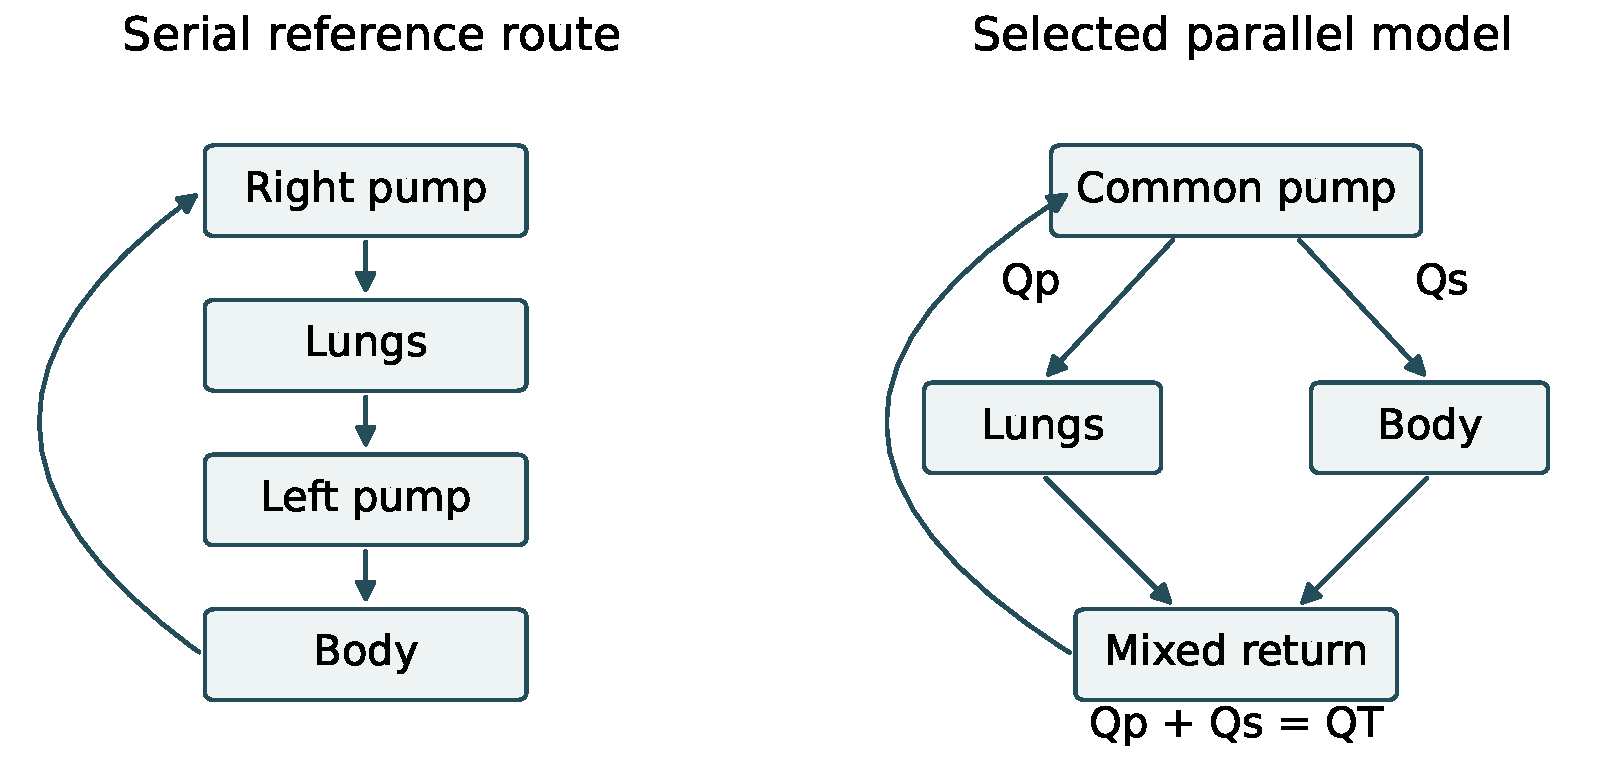
\includegraphics[width=.96\linewidth,height=.57\textheight,keepaspectratio]{circulation-routes.pdf}\par\smallskip
{\small Original route diagrams. The single-pump complete-mixing network is a selected classroom abstraction and is not a Fontan circulation. Arrows show routes, not blood color.}
\end{minipage}\end{center}
\section{Solve the parallel-flow equations}
\hypertarget{note-solve-the-parallel-flow-equations}{}\label{note:solve-the-parallel-flow-equations}
{\small \href{slides.html\#frame=three-equations-for-a-parallel-split\&step=1}{Slides for this section}}\par
Let $Q_T>0$ be a prescribed total output. The pulmonary and systemic branches have positive resistances $R_p,R_s$ and share the same pressure difference $\Delta P$. Their equations are
\[
Q_p=\frac{\Delta P}{R_p},\qquad Q_s=\frac{\Delta P}{R_s},\qquad Q_p+Q_s=Q_T.
\]
Substitution into conservation gives
\[
Q_T=\Delta P\left(\frac1{R_p}+\frac1{R_s}\right),\qquad
\Delta P=Q_T\frac{R_pR_s}{R_p+R_s}.
\]
Dividing by each branch resistance yields
\begin{equation}
Q_p=Q_T\frac{R_s}{R_p+R_s},\qquad
Q_s=Q_T\frac{R_p}{R_p+R_s}.
\end{equation}
The opposite resistance appears in each numerator because both branch laws and the total-flow constraint have been used. Equivalently, flow divides in proportion to conductance $G=1/R$.

With $Q_T=5$ L/min, $R_p=10$ and $R_s=15\ \mathrm{mmHg\,min/L}$, the common drop is $30$ mmHg, $Q_p=3$ L/min and $Q_s=2$ L/min. Both products $R_pQ_p$ and $R_sQ_s$ recover the same drop. Equal resistances give equal shares; a very large pulmonary resistance sends its share toward zero. Closing a branch is represented by zero conductance, not zero resistance.
\Needspace{10\baselineskip}

\section{Mix contents by conserving oxygen}
\hypertarget{note-mix-contents-by-conserving-oxygen}{}\label{note:mix-contents-by-conserving-oxygen}
{\small \href{slides.html\#frame=oxygen-content-has-a-transport-unit\&step=1}{Slides for this section}}\par
Let $C_p,C_s$ be oxygen contents of the returning streams, measured in mL of oxygen per liter of blood. Content is neither a partial pressure nor a saturation percentage. We prescribe $C_p=200$ and $C_s=120$ in these units; no gas-exchange or hemoglobin model calculates them here.

Over an interval $\Delta t$, incoming oxygen volumes are $Q_pC_p\Delta t$ and $Q_sC_s\Delta t$. Complete mixing produces a common outgoing content $C_m$. Equal incoming and outgoing oxygen volumes require
\[
Q_TC_m\Delta t=Q_pC_p\Delta t+Q_sC_s\Delta t.
\]
Cancel the duration and divide by the positive total flow:
\begin{equation}
C_m=\frac{Q_pC_p+Q_sC_s}{Q_T}.
\end{equation}
For the worked split, the oxygen-volume rates are $600$ and $240$ mL/min, and $C_m=840/5=168$ mL/L. The mixture must lie between the two contents because the nonnegative weights $Q_p/Q_T$ and $Q_s/Q_T$ add to one. At zero total incoming flow, this mixing equation cannot identify a concentration.
\section{Content and delivery enter as a product}
\hypertarget{note-content-and-delivery-enter-as-a-product}{}\label{note:content-and-delivery-enter-as-a-product}
{\small \href{slides.html\#frame=delivery-uses-systemic-flow\&step=1}{Slides for this section}}\par
Systemic delivery is the oxygen-volume rate entering the systemic bed:
\begin{equation}
D_s=Q_sC_m.
\end{equation}
In the first example it is $2(168)=336$ mL oxygen/min. This is delivery, not tissue consumption; consumption would also subtract the outgoing oxygen rate and require a consistent metabolic balance.

Now lower only $R_p$ from $10$ to $5$, preserving total output, systemic resistance and both return contents. The formulas give $Q_p=3.75$, $Q_s=1.25$ L/min and $C_m=180$ mL/L. Content rises, but delivery falls to $225$ mL/min.

The relationship can be made explicit by setting $x=Q_p/Q_T$. Then $Q_s=Q_T(1-x)$ and
\begin{align}
C_m&=C_s+x(C_p-C_s),\\
D_s&=Q_T(1-x)\{C_s+x(C_p-C_s)\}.
\end{align}
For the chosen contents, $D_s/Q_T=120-40x-80x^2$. If $x$ increases by a positive amount $\delta$ while remaining in $[0,1]$, the change is $-40\delta-160x\delta-80\delta^2<0$. Thus increasing the pulmonary fraction decreases systemic delivery throughout this particular fixed-content example, even while mixed content increases. This conclusion follows from the declared constants; it is not a universal rule for a physiological circulation.
\begin{center}\begin{minipage}{.98\linewidth}\centering
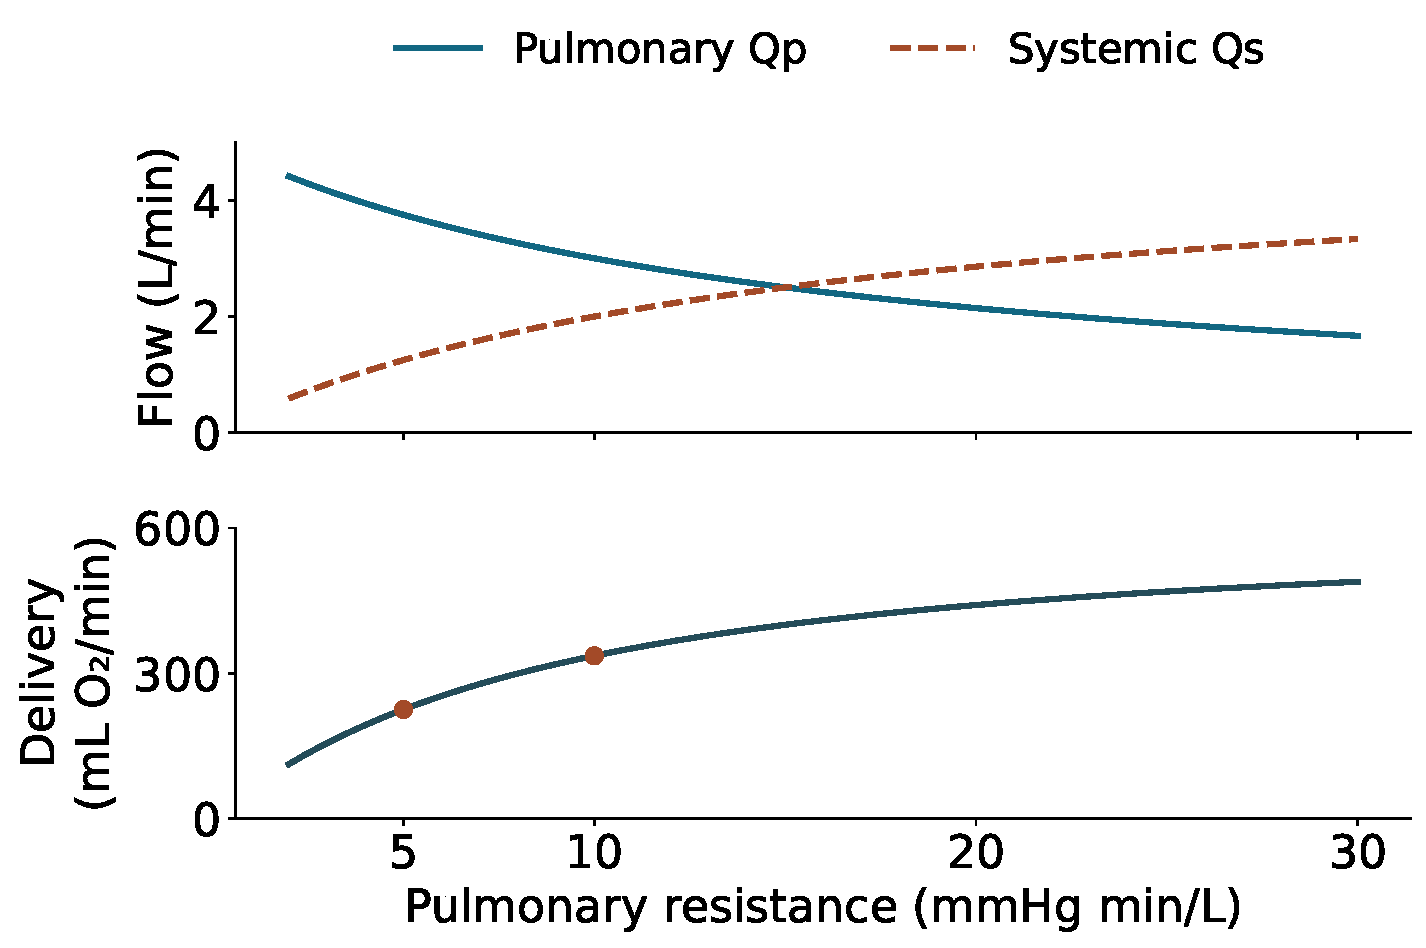
\includegraphics[width=.96\linewidth,height=.57\textheight,keepaspectratio]{flow-and-delivery.pdf}\par\smallskip
{\small QT =\allowbreak{} 5 L/min, Rs =\allowbreak{} 15 mmHg min/L, Cp =\allowbreak{} 200 and Cs =\allowbreak{} 120 mL O2/L. Only Rp changes; contents and output remain prescribed.}
\end{minipage}\end{center}
\section{Streaming, extraction, and missing oxygen dynamics}
\hypertarget{note-streaming-extraction-and-missing-oxygen-dynamics}{}\label{note:streaming-extraction-and-missing-oxygen-dynamics}
{\small \href{slides.html\#frame=close-the-accounting-then-challenge-the-assumptions\&step=1}{Slides for this section}}\par
Complete mixing is a specific assumption. Preferential streaming can make different outgoing branches receive different contents. Prescribing the return contents while changing flow also omits changes in extraction, ventilation and gas exchange. A closed oxygen-metabolism model would have to calculate those quantities rather than hold them fixed.

The branch laws, total-flow balance and oxygen balance can each be tested separately. A numerical result should satisfy $Q_p+Q_s=Q_T$, equal branch pressure drops, and equality of incoming and outgoing oxygen-volume rates. Passing those tests establishes consistency of the abstraction. It cannot identify an appropriate patient-specific resistance, surgical outcome or target saturation. A focused project can instead state the chosen network and compare which conclusion survives when one of its fixed quantities becomes a modeled variable.
\bigskip
\section*{Exercises}
\par\noindent\begin{minipage}{\linewidth}
\subsection*{MC05-E1. A signed connection}
A passive shunt has a positive arrow from A to B and resistance 4 mmHg min/L.

\textbf{a} For PA =\allowbreak{} 14 and PB =\allowbreak{} 6 mmHg, find flow and direction.

\end{minipage}\par\medskip
\textbf{b} Increase both pressures by 5 mmHg. Recompute flow and explain.

\textbf{c} Set PA =\allowbreak{} 6 and PB =\allowbreak{} 14. Find signed flow and explain why a resistor may not represent a valve.

\par\noindent\begin{minipage}{\linewidth}
\subsection*{MC05-E2. Check parallel flow and mixing}
Use QT =\allowbreak{} 6 L/min, Rp =\allowbreak{} 20 and Rs =\allowbreak{} 10 mmHg min/L. Prescribe Cp =\allowbreak{} 210 and Cs =\allowbreak{} 120 mL O2/L; assume complete mixing.

\textbf{a} Find Qp and Qs and verify the common pressure drop.

\end{minipage}\par\medskip
\textbf{b} Find mixed content, showing the oxygen-volume balance.

\textbf{c} Find systemic delivery and name two biological processes omitted by prescribing return contents.

\par\noindent\begin{minipage}{\linewidth}
\subsection*{MC05-E3. Challenge an attractive conclusion}
A report says: ``Our resistance change raised the mixed oxygen content, therefore it improved systemic oxygen delivery.''

\textbf{a} Give a numerical counterexample using two positive flows and contents of your choosing.

\end{minipage}\par\medskip
\textbf{b} State a bounded project question and two quantities to hold fixed.

\textbf{c} Name one model check and one independent observation needed before interpreting the model physiologically.

\section*{References}
\noindent\begin{minipage}{\linewidth}
Zan Ahmad, Fall 2023 HEART syllabus. Public PDF pp. 1--2, Course Topics and Course Expectations; editable syllabus pp. 2--3, project requirements.

\end{minipage}\par\medskip
\noindent\begin{minipage}{\linewidth}
Hoppensteadt and Peskin, Modeling and Simulation in Medicine and the Life Sciences, second edition. Printed pp. 28--30; PDF pp. 41--43, section 1.10 shunt topology and junction balances.

\end{minipage}\par\medskip
\noindent\begin{minipage}{\linewidth}
Rychik et al. (2019), Evaluation and Management of the Child and Adult With Fontan Circulation: A Scientific Statement From the American Heart Association. Circulation 140, e234--e284; circulation and staged-palliation background.

\url{https://www.ahajournals.org/doi/10.1161/CIR.0000000000000696}
\end{minipage}\par\medskip
\end{document}
